\let\negmedspace\undefined
\let\negthickspace\undefined
\documentclass[journal]{IEEEtran}
\usepackage[a5paper, margin=10mm, onecolumn]{geometry}
%\usepackage{lmodern} % Ensure lmodern is loaded for pdflatex
\usepackage{tfrupee} % Include tfrupee package

\setlength{\headheight}{1cm} % Set the height of the header box
\setlength{\headsep}{0mm}     % Set the distance between the header box and the top of the text

\usepackage{gvv-book}
\usepackage{gvv}
\usepackage{cite}
\usepackage{amsmath,amssymb,amsfonts,amsthm}
\usepackage{algorithmic}
\usepackage{graphicx}
\usepackage{textcomp}
\usepackage{xcolor}
\usepackage{txfonts}
\usepackage{listings}
\usepackage{enumitem}
\usepackage{mathtools}
\usepackage{gensymb}
\usepackage{comment}
\usepackage[breaklinks=true]{hyperref}
\usepackage{tkz-euclide} 
\usepackage{listings}
% \usepackage{gvv}                                        
\def\inputGnumericTable{}                                 
\usepackage[latin1]{inputenc}                                
\usepackage{color}                                            
\usepackage{array}                                            
\usepackage{longtable}                                       
\usepackage{calc}                                             
\usepackage{multirow}                                         
\usepackage{hhline}                                           
\usepackage{ifthen}                                           
\usepackage{lscape}
\begin{document}

\bibliographystyle{IEEEtran}
\vspace{3cm}
\title{9.3.12}
\author{EE24BTECH11028 - Jadhav Rajesh}
% \maketitle
% \newpage
% \bigskip
{\let\newpage\relax\maketitle}

\renewcommand{\thefigure}{\theenumi}
\renewcommand{\thetable}{\theenumi}
\setlength{\intextsep}{10pt} % Space between text and floats


\numberwithin{equation}{enumi}
\numberwithin{figure}{enumi}
\renewcommand{\thetable}{\theenumi}
\textbf{Question:} Which of the following differential equations has $y = x$ as one of its particular solution?\\
 \begin{align}
 \brak{C}  \frac{d^{2}y}{dx^{2}}-x^{2}\frac{dy}{dx}+xy=0
 \end{align}
                         
 \solution 
 \textbf{NUMERICAL METHOD}\\
	
Consider,
\begin{align}
\frac{d^2y}{dx^2} - x^2\frac{dy}{dx} + xy = 0
\end{align}

Assuming the initial conditions $y(0) = 0$ and $y'(0) = 1.$


\textbf{HOMOGENEOUS PART:}\\

The associated homogeneous equation is:
\begin{align}
\frac{d^2y}{dx^2} - x^2\frac{dy}{dx} + xy = 0.
\end{align}

Assume a power series solution:
\begin{align}
y_h = \sum_{n=0}^\infty a_n x^n.
\end{align}

The derivatives are:
\begin{align}
\frac{dy_h}{dx} = \sum_{n=1}^\infty n a_n x^{n-1}, \quad 
\frac{d^2y_h}{dx^2} = \sum_{n=2}^\infty n(n-1)a_n x^{n-2}.
\end{align}

Substitute into the homogeneous equation:
\begin{align}
\sum_{n=2}^\infty n(n-1)a_n x^{n-2} - x^2 \sum_{n=1}^\infty n a_n x^{n-1} + x \sum_{n=0}^\infty a_n x^n = 0.
\end{align}

Rewriting terms, we derive the recurrence relation:
\begin{align}
a_{n+2} = \frac{n-2}{(n+2)(n+1)}a_{n-1}.
\end{align}

Apply the initial conditions\\

The initial conditions are:
$y(0) = 0 \quad \Rightarrow \quad a_0 = 0,$\\
$y'(0) = 1 \quad \Rightarrow \quad a_1 = 1.$

Using the recurrence relation:
\begin{align}
a_{n+2} = \frac{n-2}{(n+2)(n+1)}a_{n-1},
\end{align}

we compute the coefficients:

\begin{enumerate}
    \item For $n = 0$: $a_0 = 0$
    \item For $n = 1$: $a_1 = 1$
    \item For $n = 2$: $a_2 = \frac{0 - 2}{(2+2)(2+1)}a_1 = \frac{-2}{12} = -\frac{1}{6}$
    \item For $n = 3$: $a_3 = \frac{1 - 2}{(3+2)(3+1)}a_2 = \frac{-1}{20}.\brak{-\frac{1}{6}} = \frac{1}{120}$
    \item For $n = 4$: $a_4 = \frac{2 - 2}{(4+2)(4+1)}a_3 = 0$
\end{enumerate}

The pattern is:
\begin{align}
a_{2k} = 0, \quad a_{2k+1} = \frac{(-1)^k}{(2k+1)!}.
\end{align}

Therefore, the homogeneous solution is:
\begin{align}
y= \sum_{k=0}^\infty \frac{(-1)^k x^{2k+1}}{(2k+1)!}.
\end{align}
\begin{figure}[h!]
   \centering
   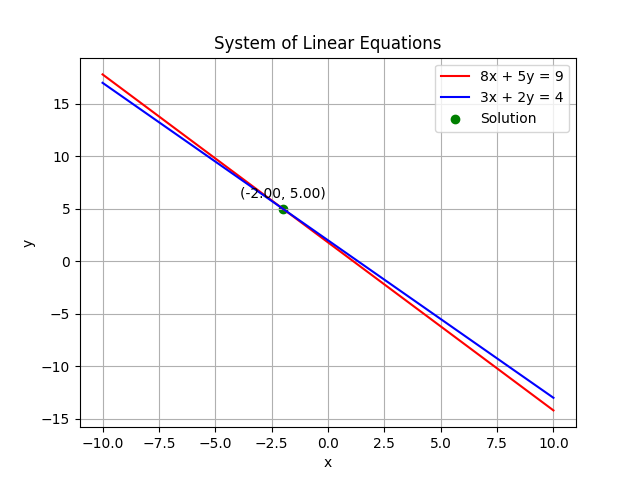
\includegraphics[width=1\columnwidth]{figure/fig.png} 
   \caption{Numerical Solution}
   \label{stemplot}
\end{figure}

\end{document}
